\section{Chaotisches Verhalten}
Wie im vorherigen Kapitel angedeutet, wurde mithilfe der Gleichungen eine Simulation erstellt,
um das chaotische Verhalten näher zu untersuchen.
Diese Simulation wurde von Alex Krieg, einem Studenten der Fachhochschule OST, entwickelt.
\index{Alex Krieg}%
\index{Krieg, Alex}%
Die daraus gewonnenen Erkenntnisse werden in diesem Abschnitt erläutert.

\begin{figure}
    \centering
    \begin{minipage}{0.45\textwidth}
        \centering
        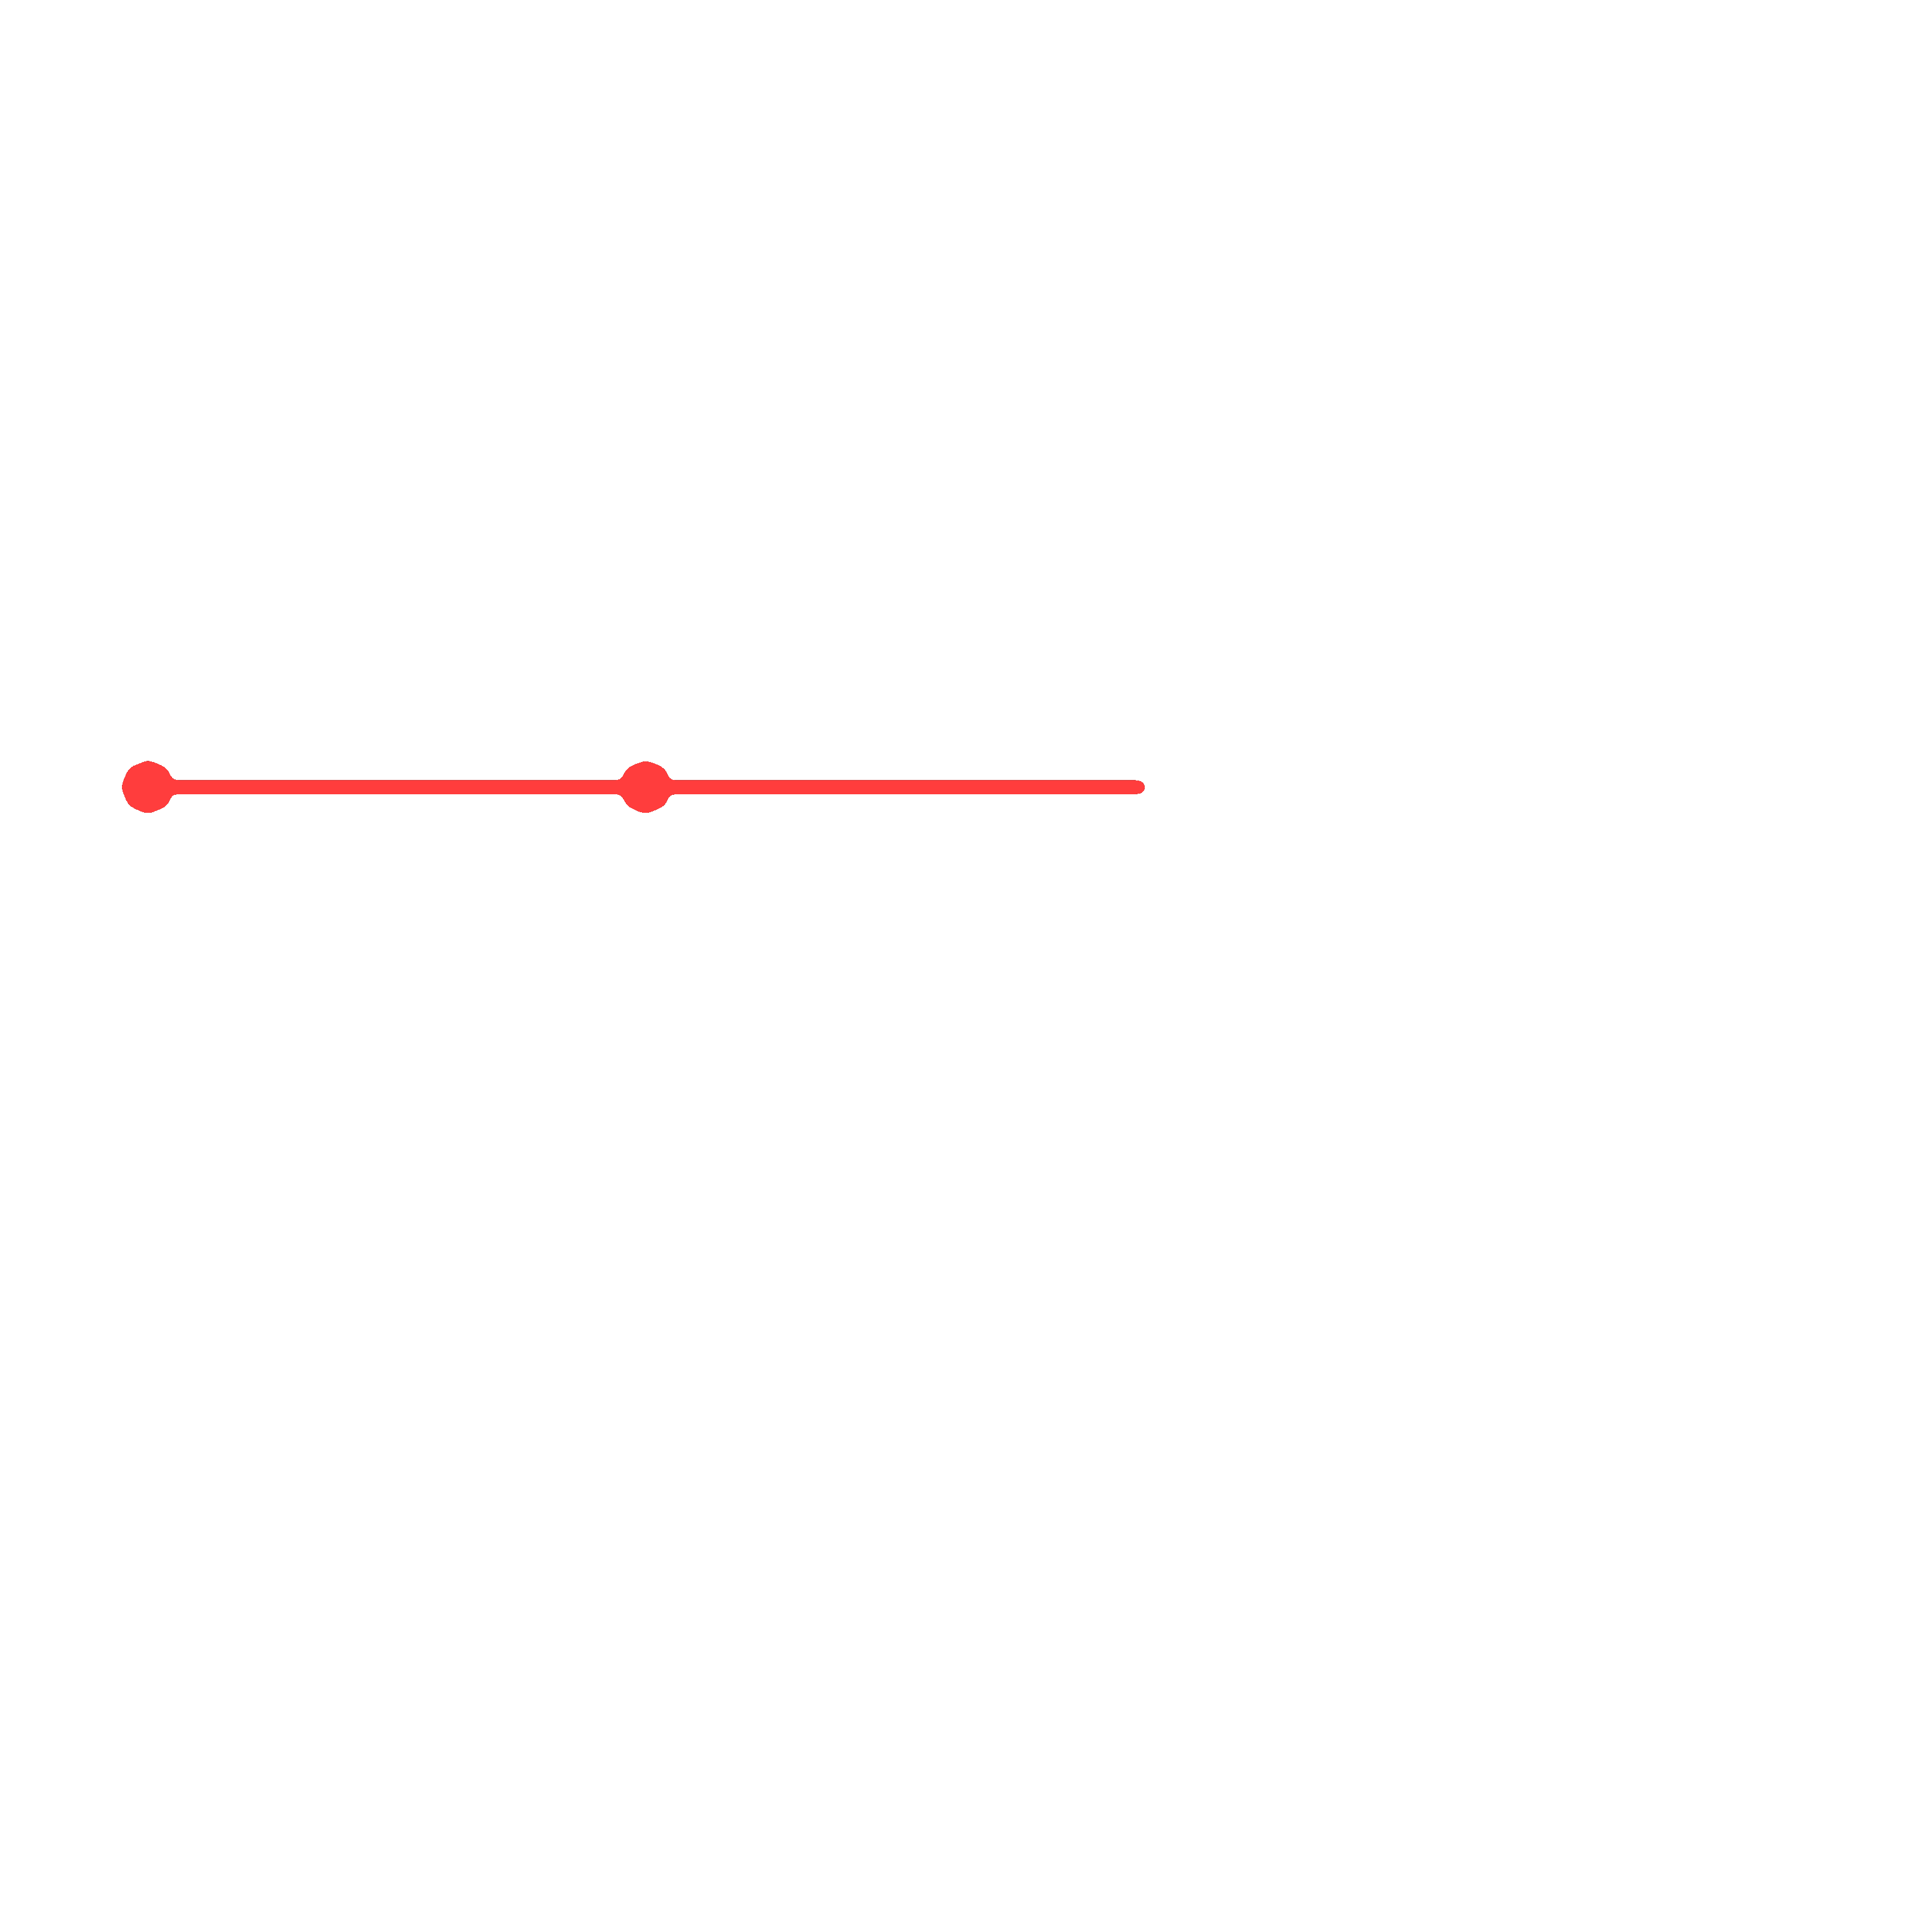
\includegraphics[width=\textwidth]{papers/doppelpendel/images/pendel_stand_90.png}
    \end{minipage}
    \hfill
    \begin{minipage}{0.45\textwidth}
        \centering
        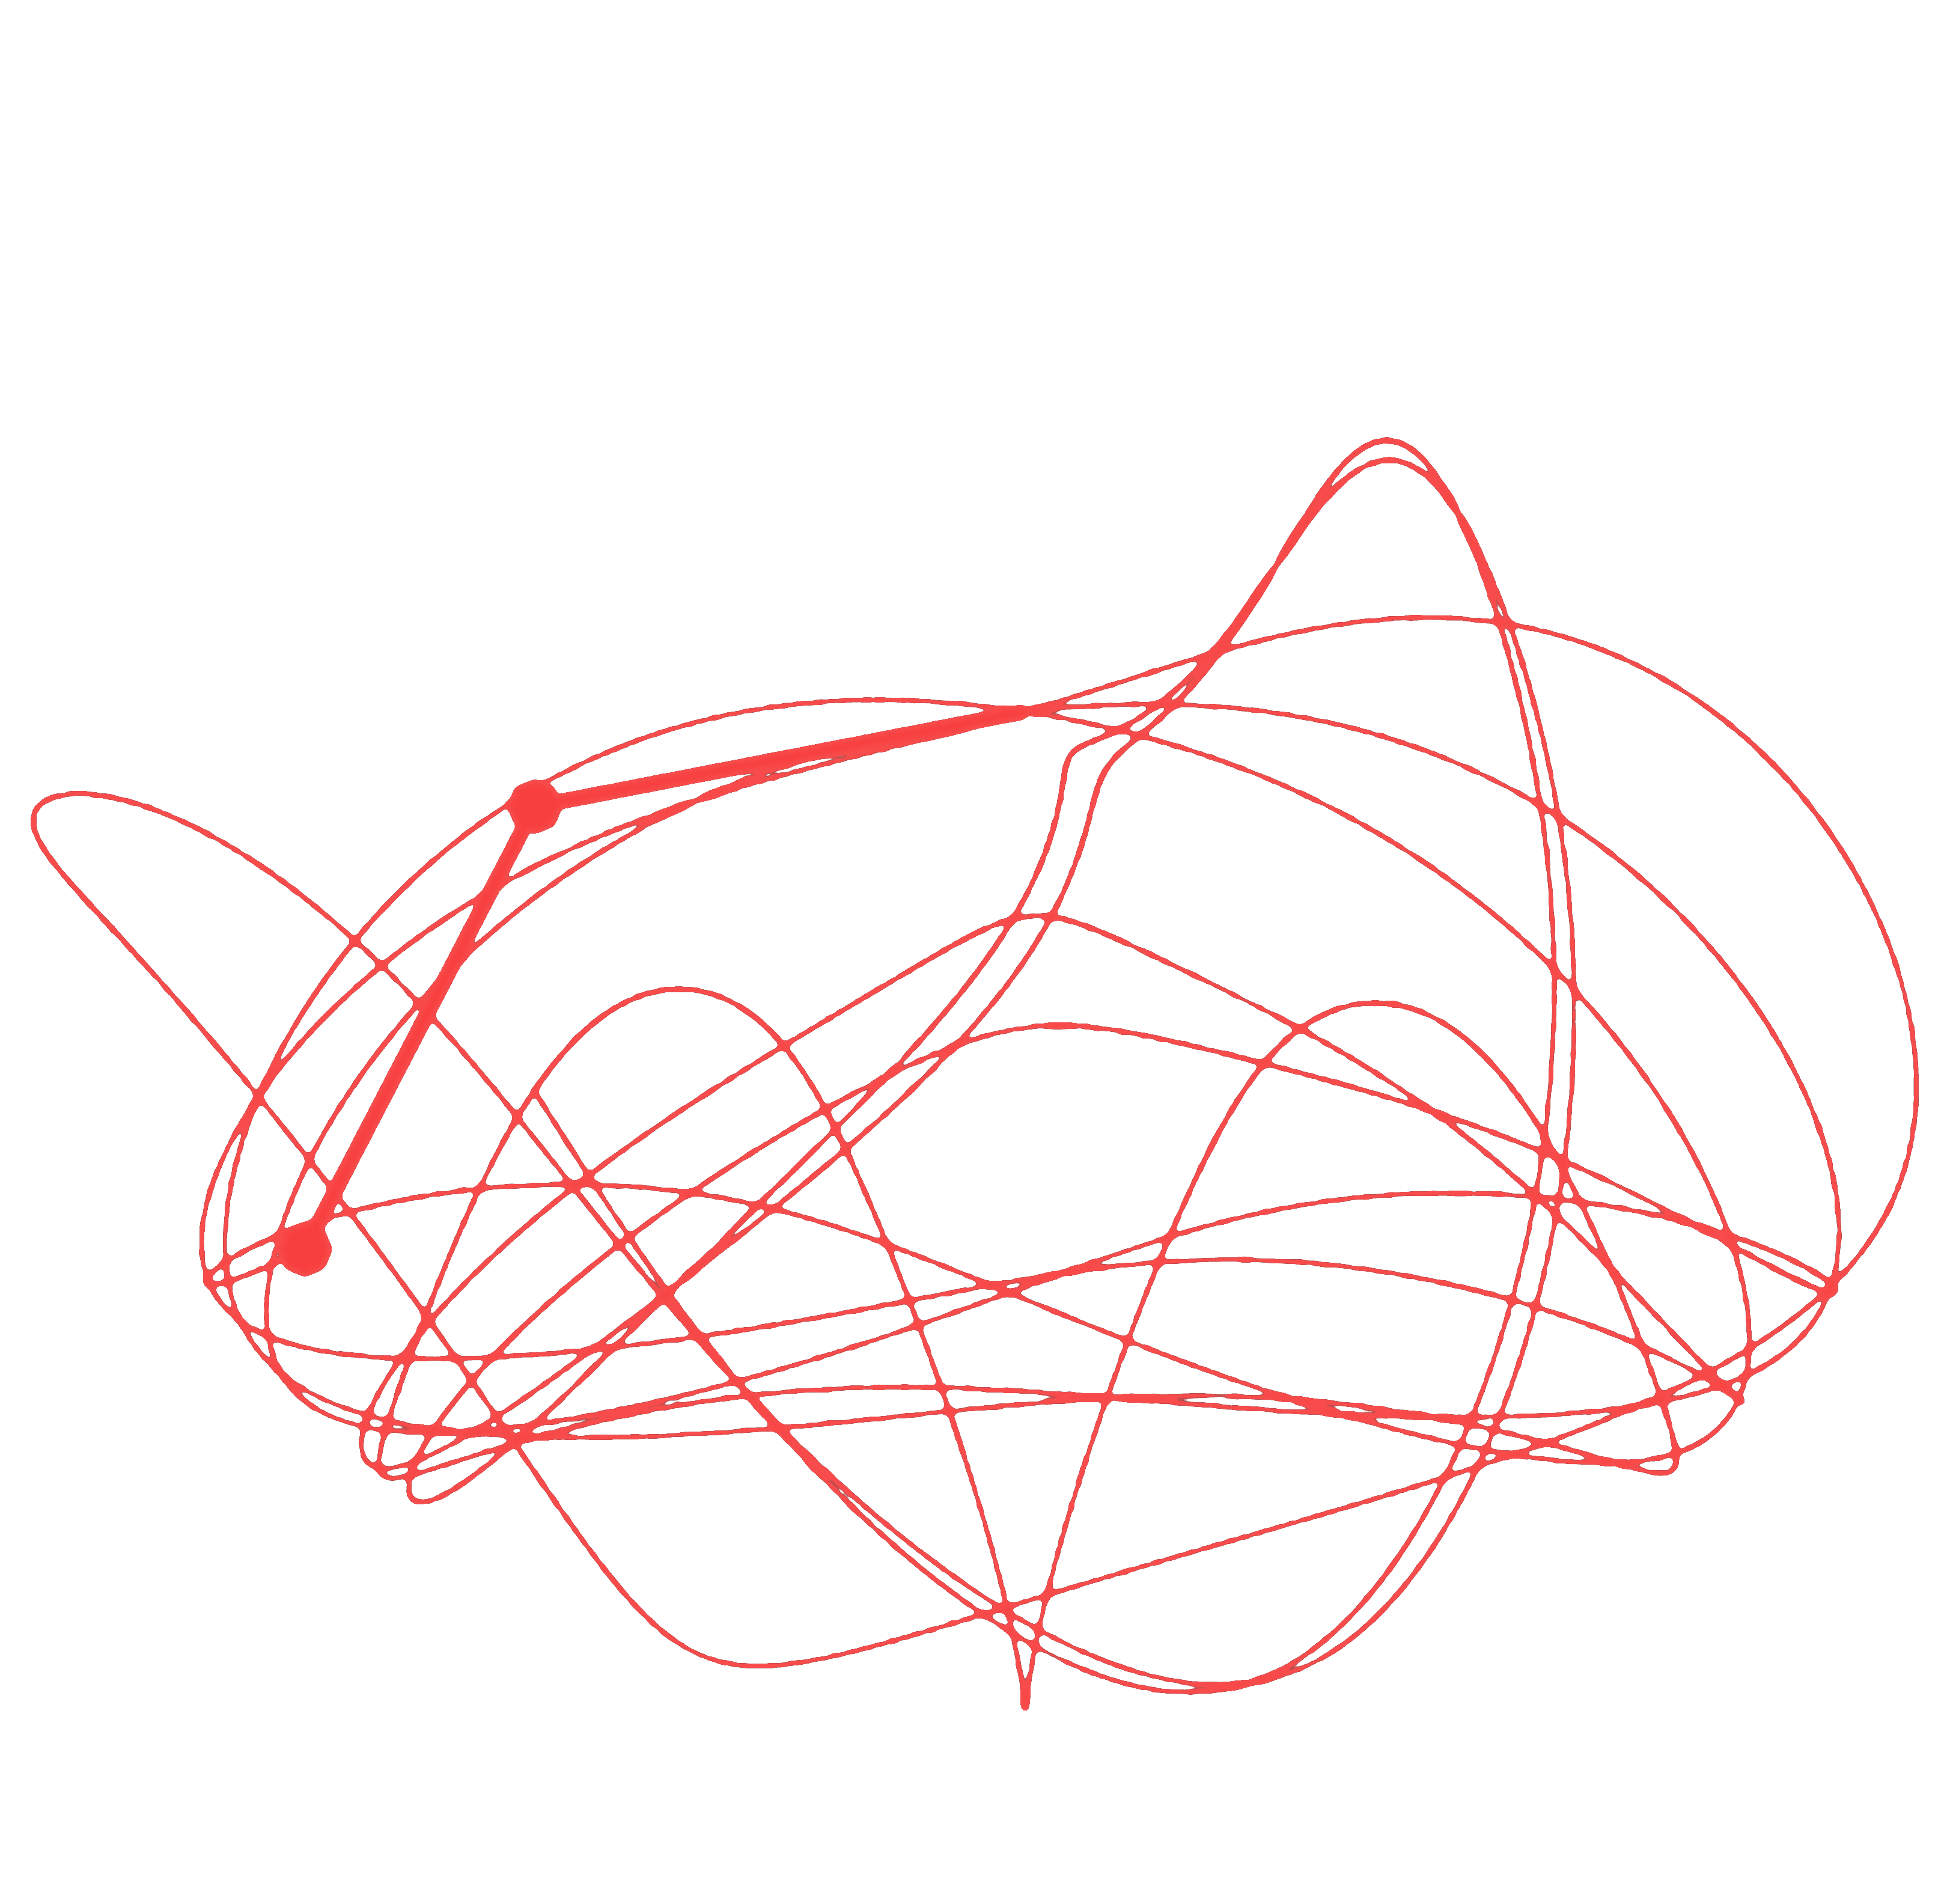
\includegraphics[width=\textwidth]{papers/doppelpendel/images/pendel_spur_90.png}
    \end{minipage}
    \caption{Pendel mit der Anfangsbedingung 90°.}
    \label{fig:pendel_bei_90}
    \centering
    \begin{minipage}{0.45\textwidth}
        \centering
        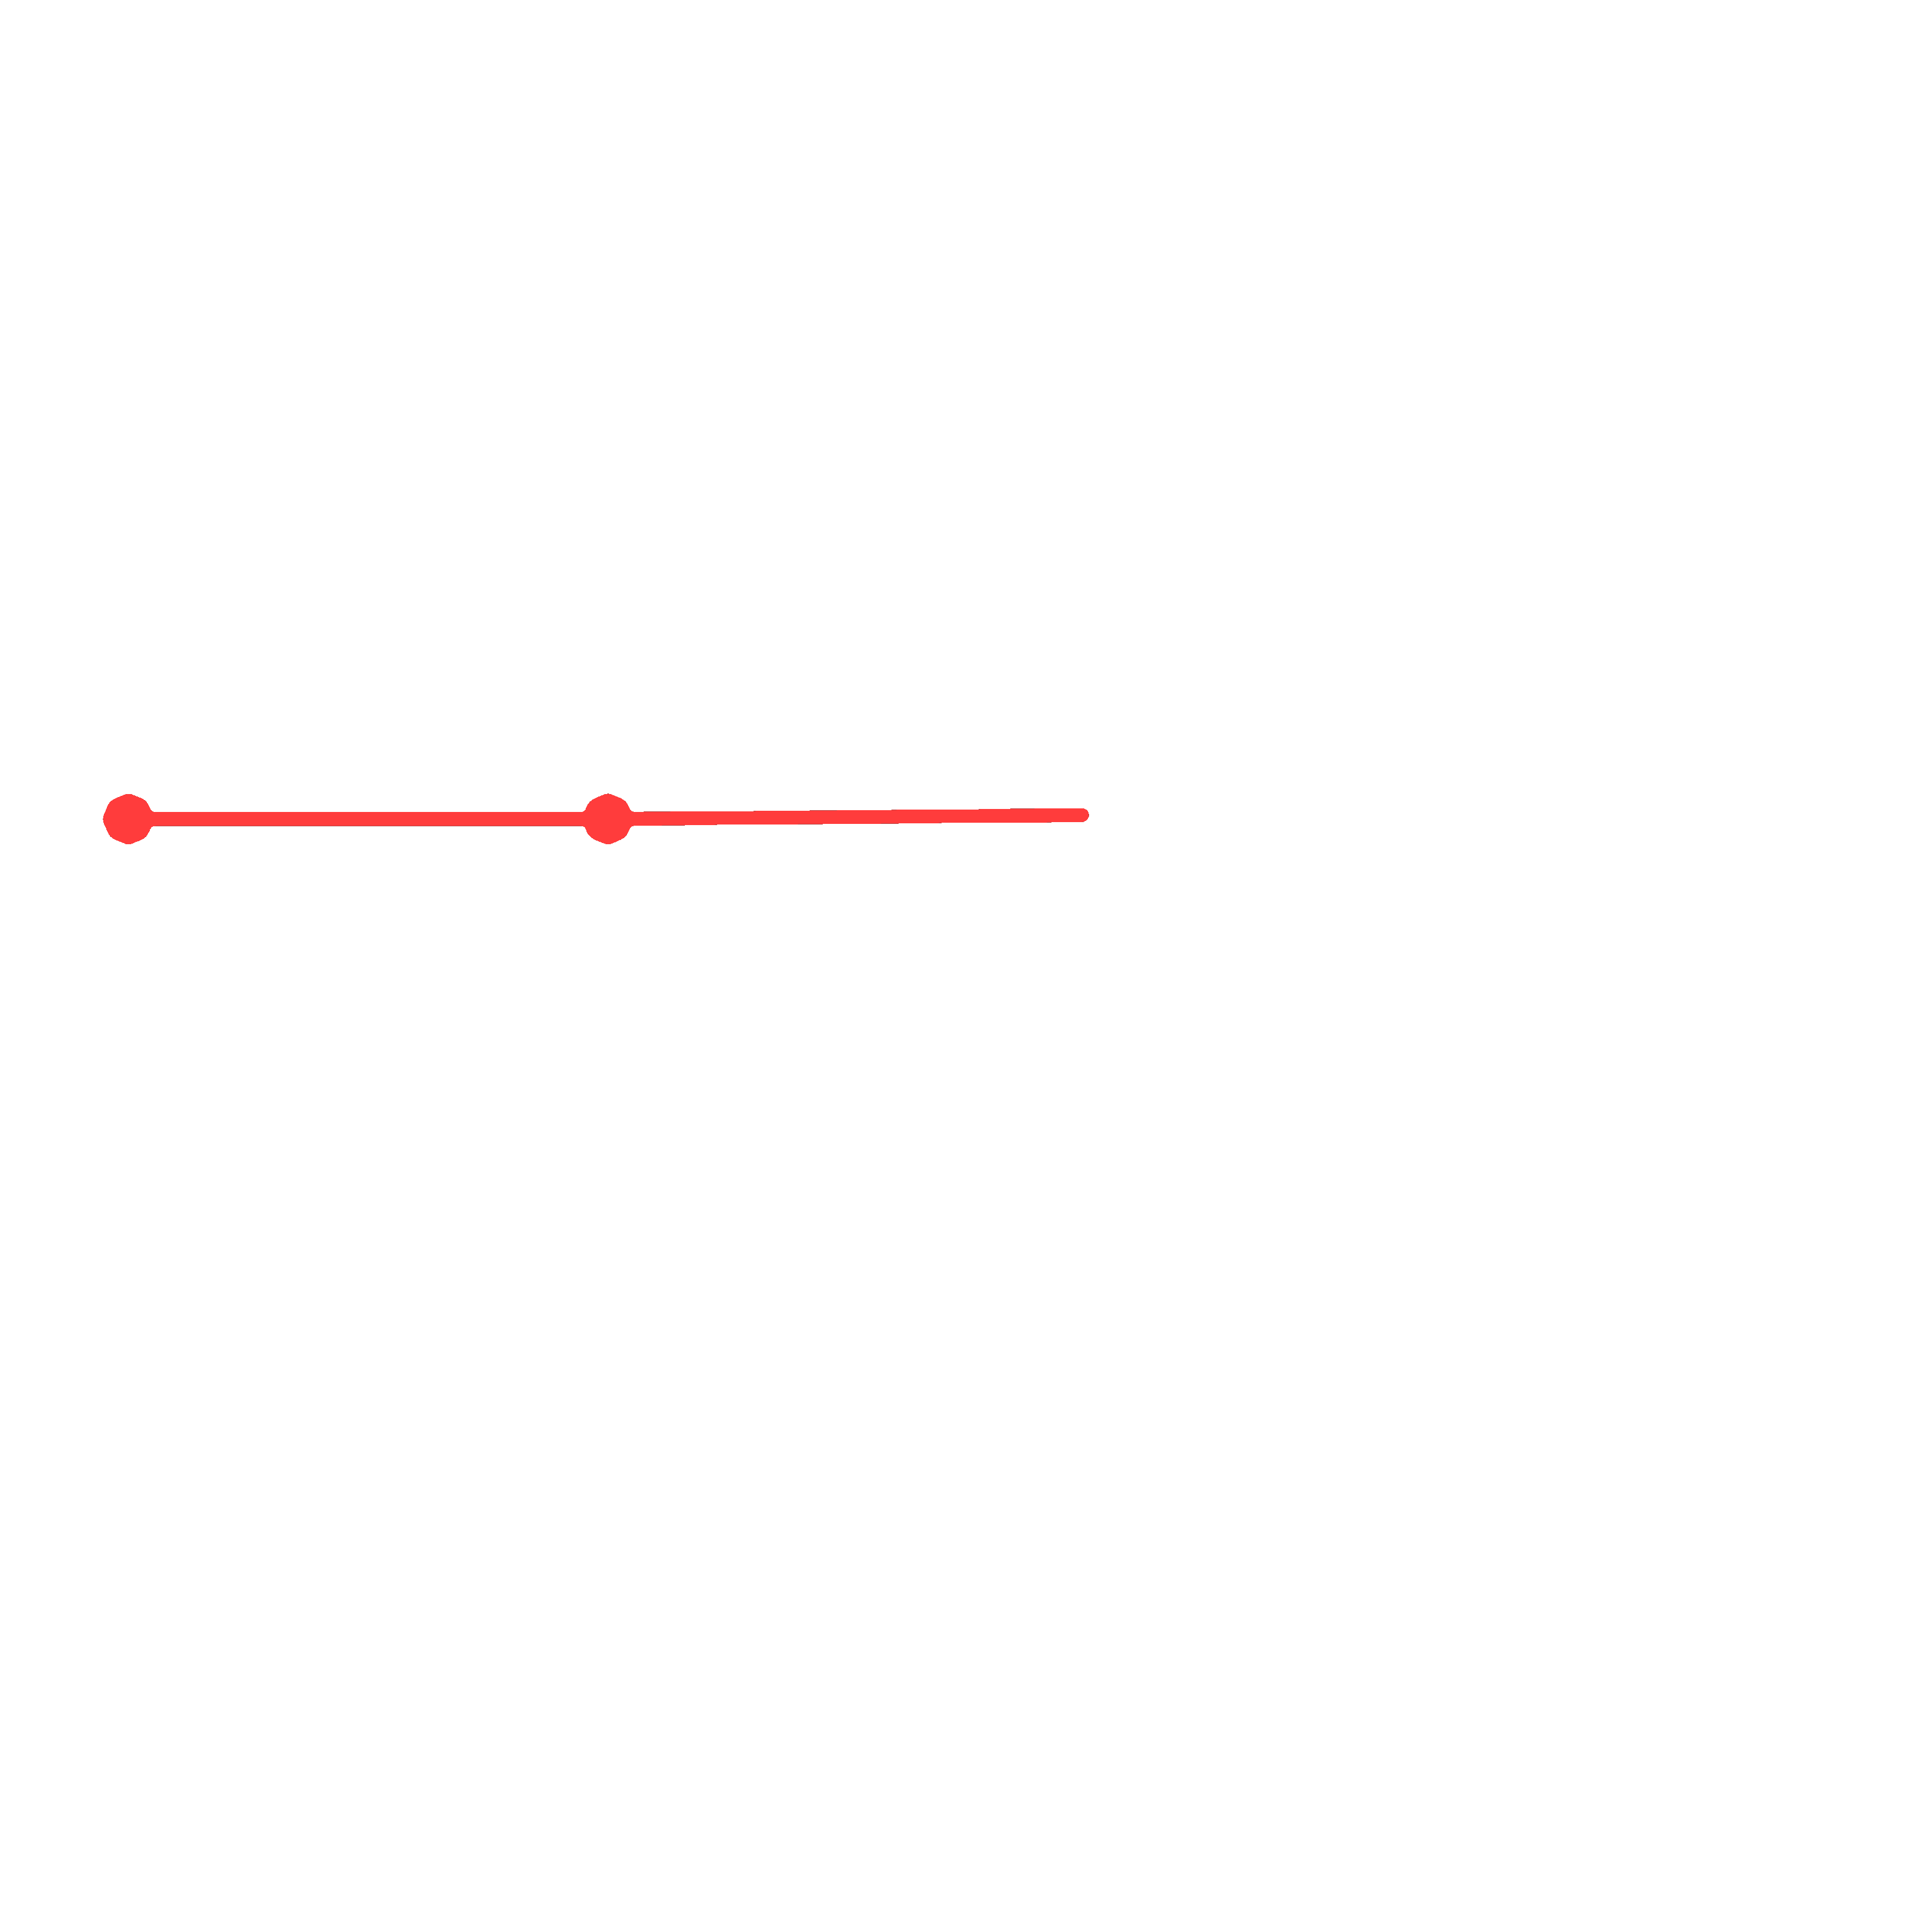
\includegraphics[width=\textwidth]{papers/doppelpendel/images/pendel_stand_kleiner_90.png}
    \end{minipage}
    \hfill
    \begin{minipage}{0.45\textwidth}
        \centering
        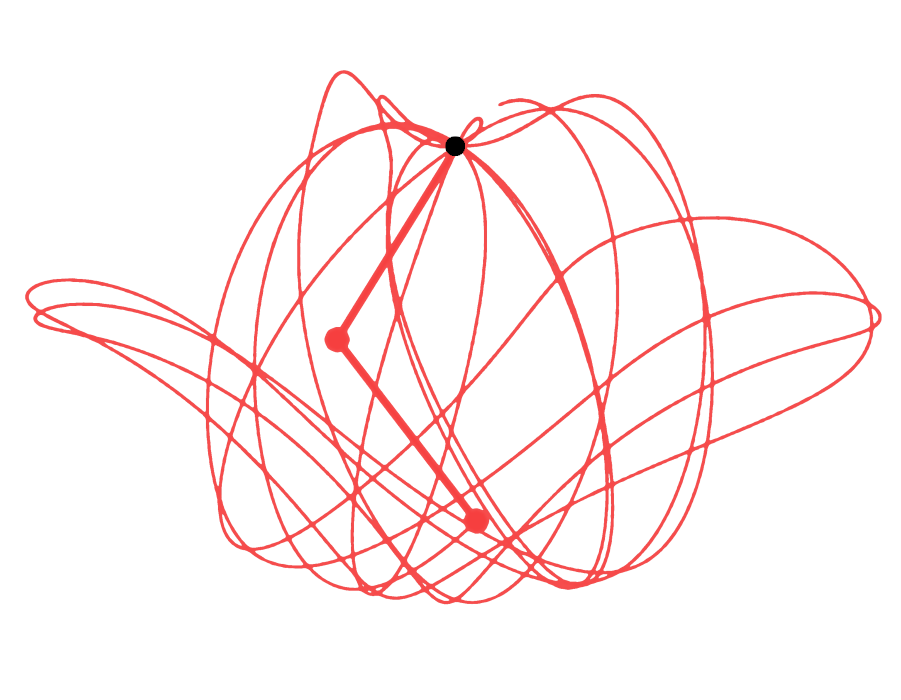
\includegraphics[width=\textwidth]{papers/doppelpendel/images/pendel_spur_kleiner_90.png}
    \end{minipage}
    \caption{Anfangsbedingung der Winkel ist kaum sichtbar kleiner als 90°.}
    \label{fig:pendel_bei_weniger_90}
    \centering
    \begin{minipage}{0.45\textwidth}
        \centering
        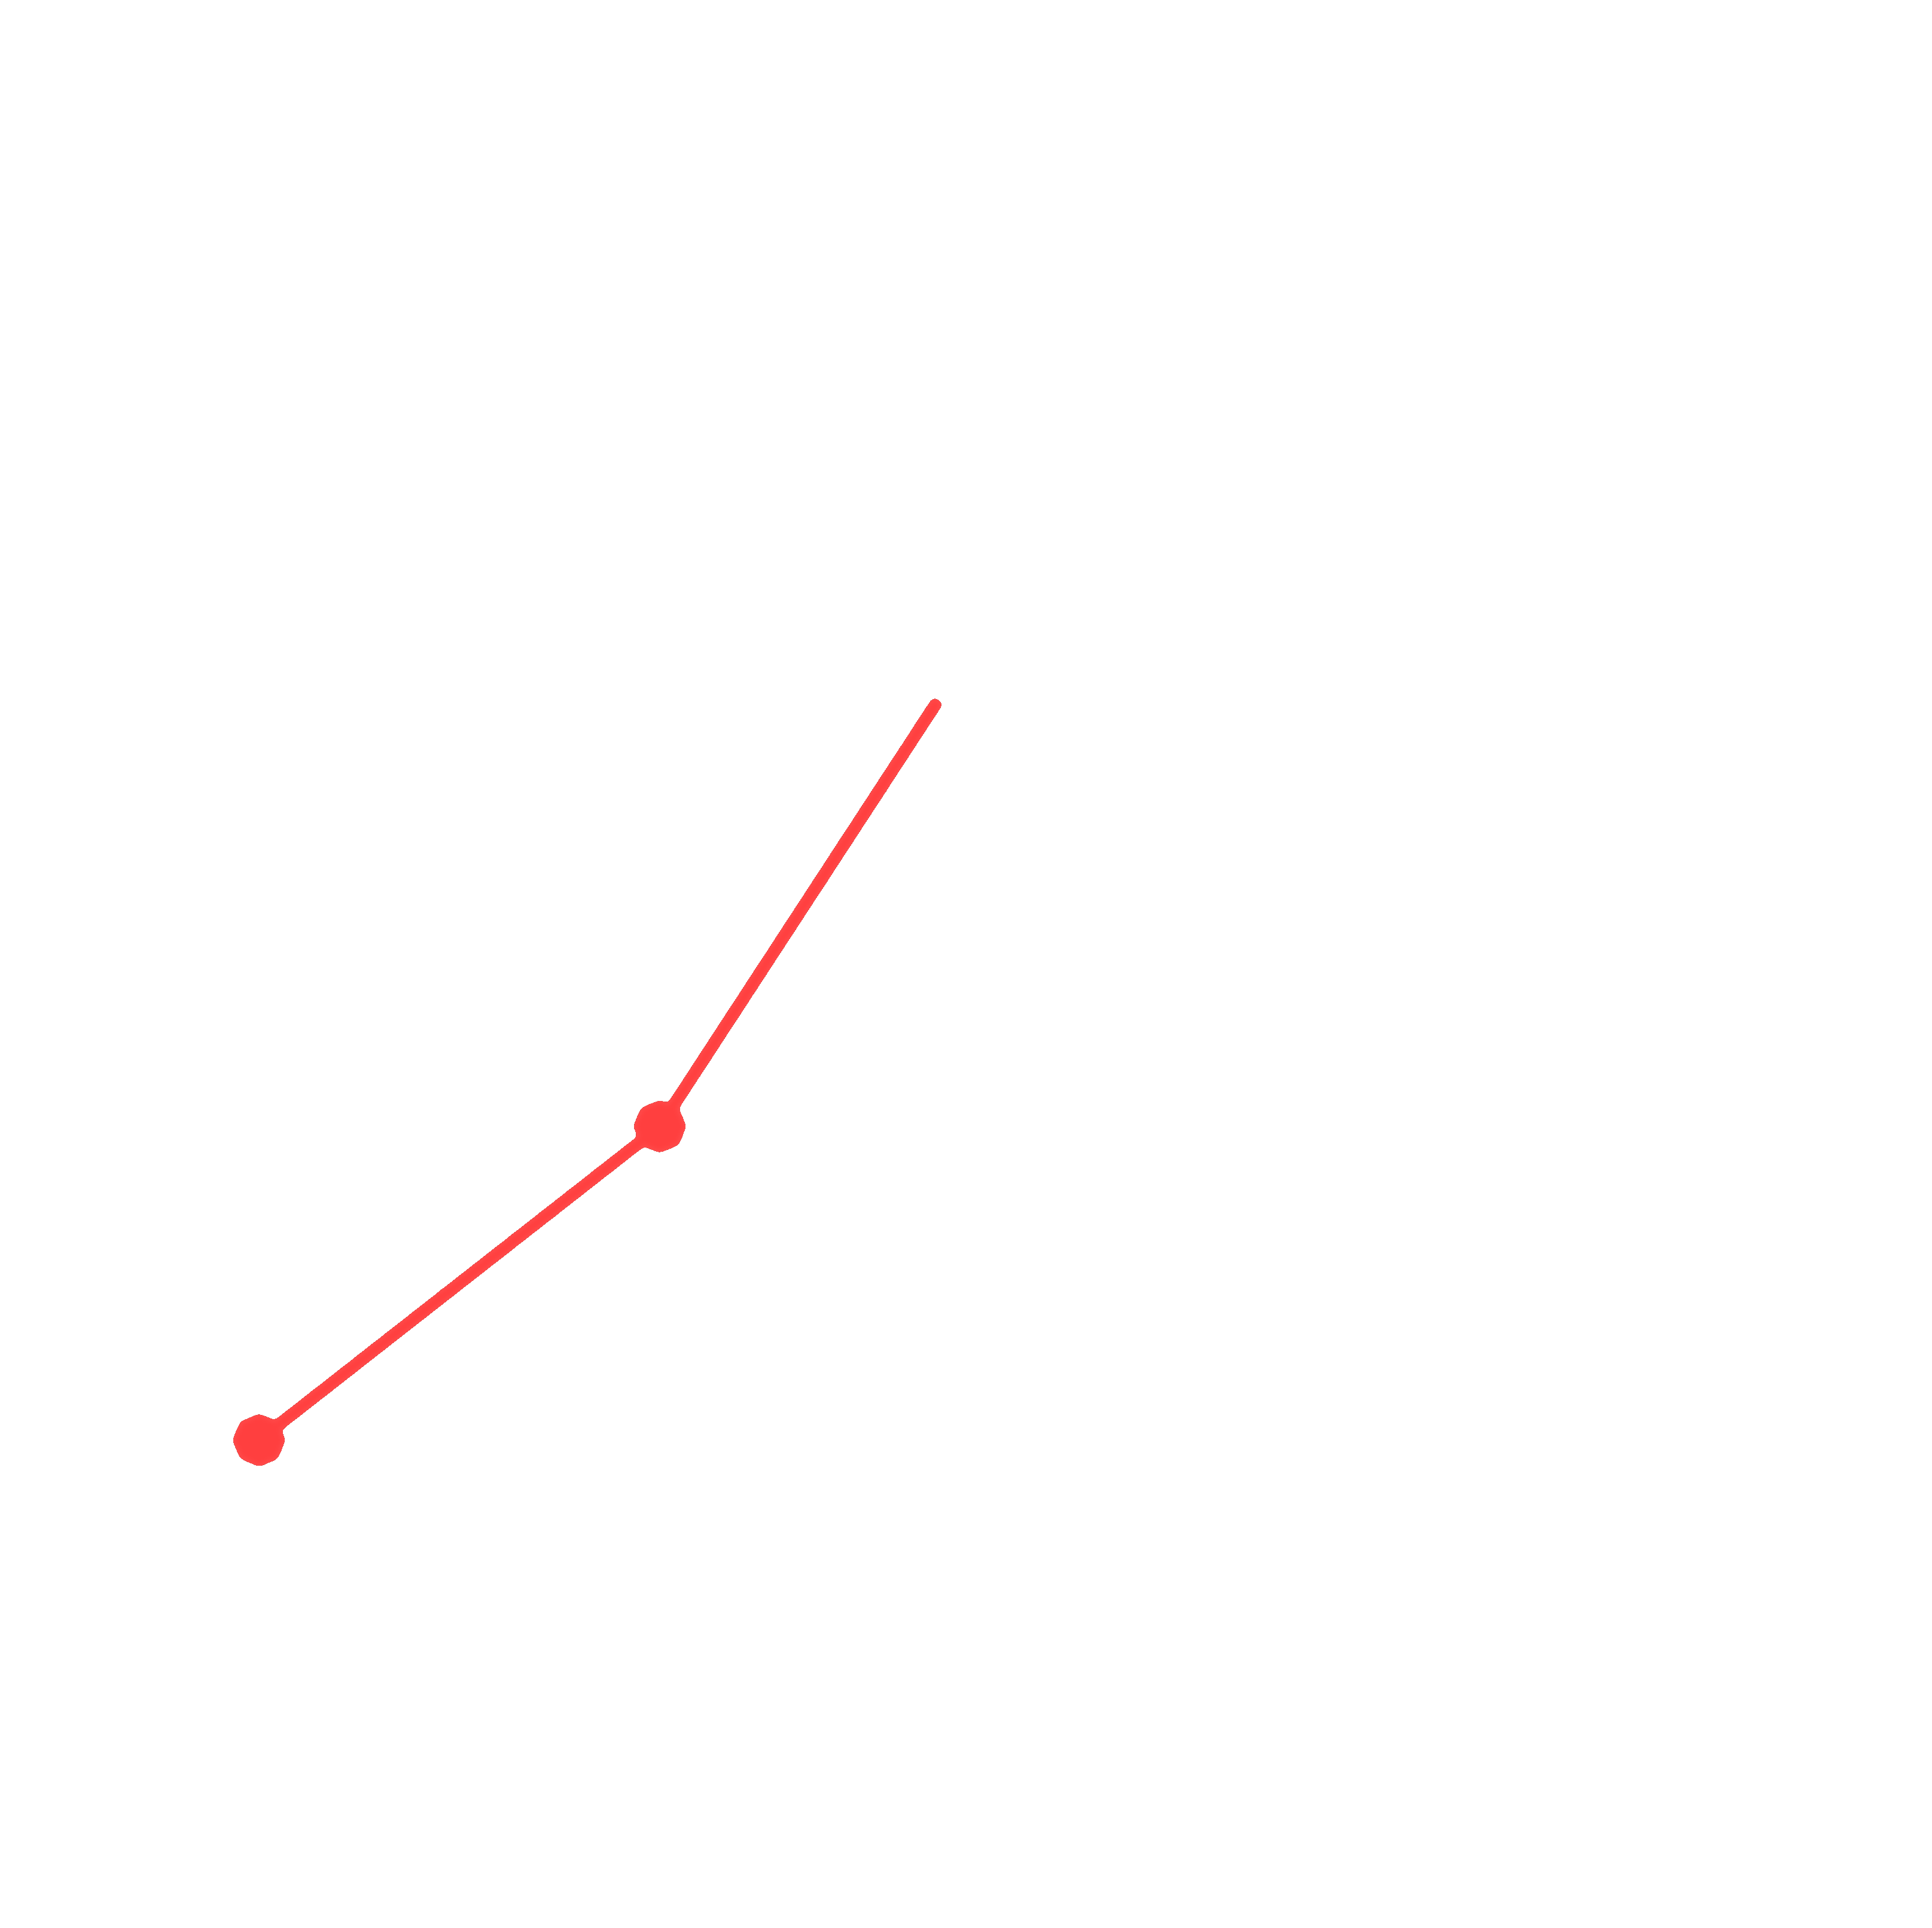
\includegraphics[width=\textwidth]{papers/doppelpendel/images/pendel_stand_nichtchaotisch.png}
    \end{minipage}
    \hfill
    \begin{minipage}{0.45\textwidth}
        \centering
        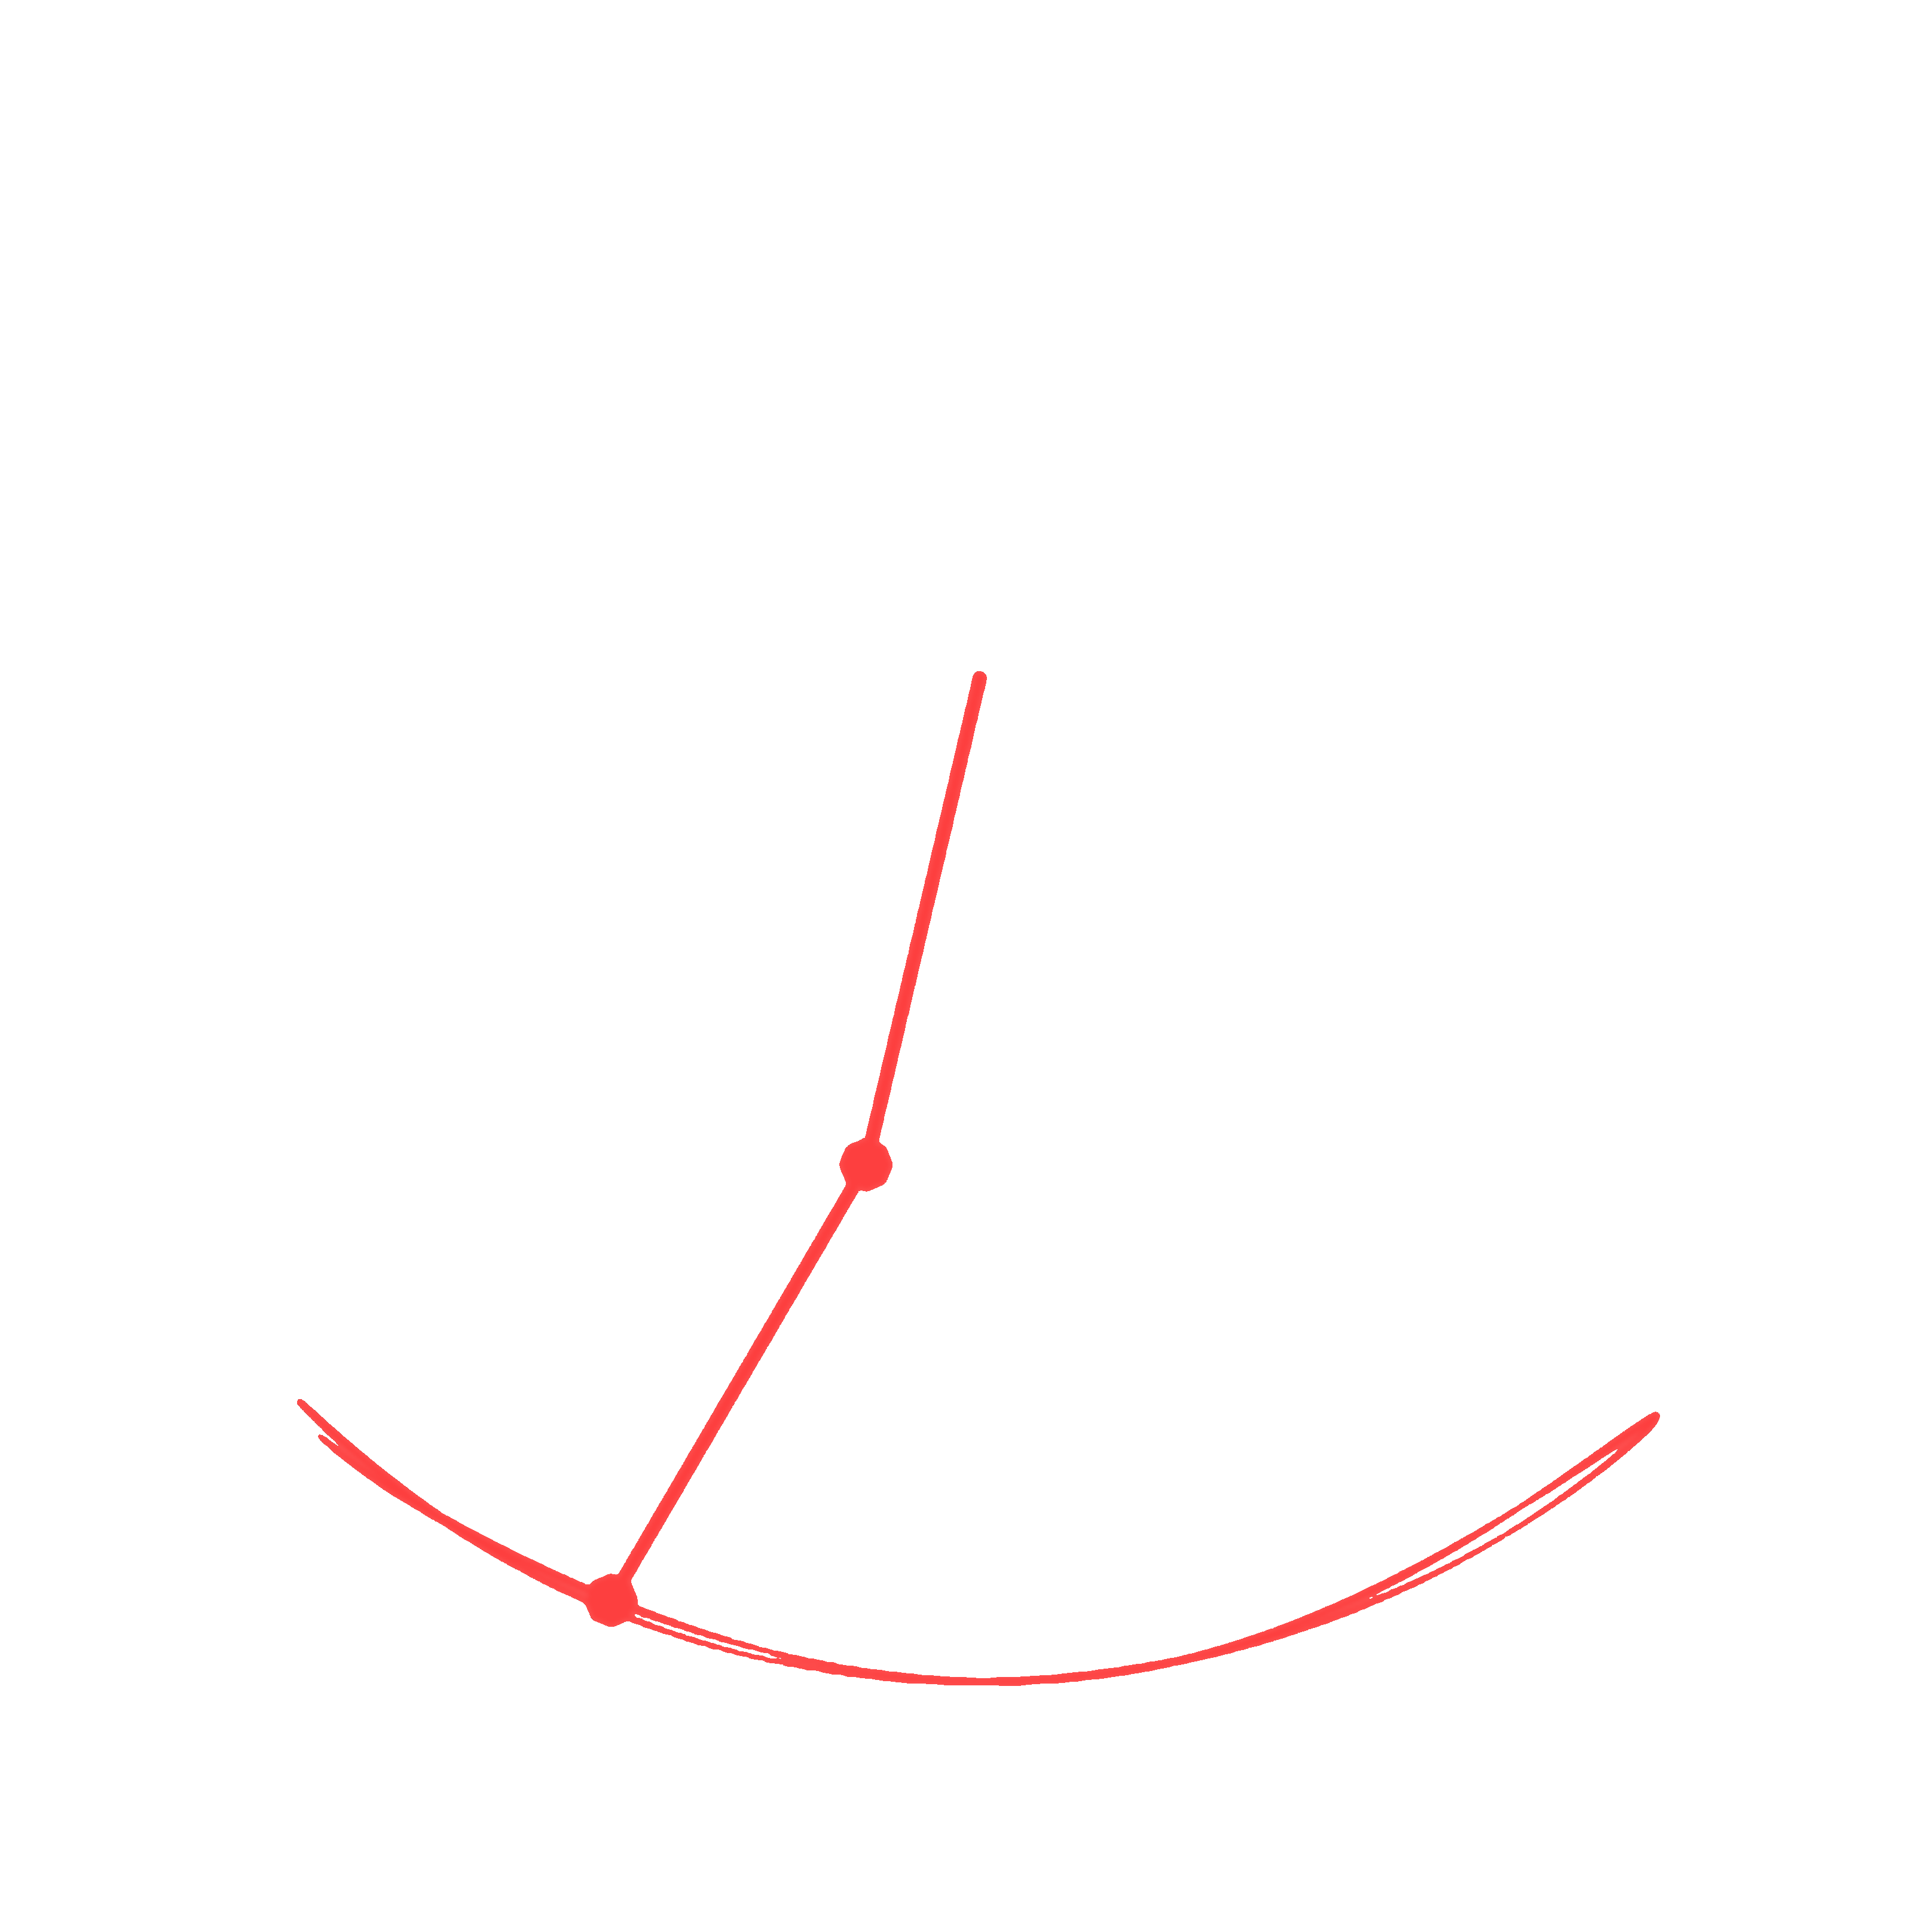
\includegraphics[width=\textwidth]{papers/doppelpendel/images/pendel_spur_nichtchaotisch.png}
    \end{minipage}
    \caption{Pendel wird nicht chaotisch, aufgrund kleiner Winkel.}
    \label{fig:pendel_nichtchaotisch}
\end{figure}

\subsection{Physikalisches Chaos}
In der Physik wird das Chaos als aperiodisches Langzeitverhalten in einem deterministischen
\index{aperiodisch}%
\index{Langzeitverhalten}%
System bezeichnet, mit empfindlicher Abhängigkeit der Anfangsbedingungen.
\index{empfindliche Abhängigkeit}%
\index{Anfangsbedingungen}%
Aperiodisches Langzeitverhalten bedeutet, wenn sich das System nach langer zeitlicher Betrachtung
nicht periodisch wird.
Das einfache Pendel weist ein periodisches Langzeitverhalten auf,
denn es schwingt immer im gleichen Muster.
Deterministisch heisst im übertragenen Sinn, dass das Verhalten des Systems gleich bleibt,
sofern die Anfangsbedingungen die Gleichen sind.
Trotzdem kann sich bei der kleinsten Abweichung eine völlig andere Trajektorie bilden.
Dies rührt daher, dass die immer vorhandenen kleinen Störungen, wie z.~B.~thermisches Rauschen,
\index{Rauschen}%
\index{thermisch}%
bei empfindlicher Abhängigkeit der Anfangsbedingung, die Bahn deutlich beeinflussen.
Dieses Phänomen ist auch bekannt als der Schmetterlingseffekt \cite{doppelpendel:schmetterlingseffekt}.
\index{Schmetterlingseffekt}%

\subsection{Simulationsanalyse}
Im ersten Experiment wollen wir uns ansehen, wie die Trajektorie eines Pendels aussieht,
welche aus der horizontalen Lage bzw. Anfangsbedingung 90° startet
(siehe Abbildung \ref{fig:pendel_bei_90}).
Beim Wiederholen dieses Experiment lässt sich feststellen, dass für exakt dieselben Anfangsbedingungen
das gleiche Ergebnis resultiert und daher deterministisch ist.

Im zweiten Experiment (Abbildung \ref{fig:pendel_bei_weniger_90}), wurde die vorherige
Anfangsbedingung marginal verändert.
\(\vartheta_2\) wurde um ca.~ein Zehntel Grad verringert.
Nichtsdestotrotz lässt sich am Resultat nichts wiedererkennen.

Im letzten Experiment (Abbildung \ref{fig:pendel_nichtchaotisch}) wird gezeigt,
wie das Pendel bei kleineren Winkeln nicht chaotisch wird.
Es lässt bereits vermuten, dass die Pendel mit hoher potentieller Energie eine stärkere Tendenz haben,
in den chaotischen Zustand überzugehen.
Das zeigen auch die Trajektoren aus diesen Versuchen.

Was wir hier für drei verschiedene Anfangsbedingungen durchgeführt haben, kann man selbstverständlich
für etliche Winkel durchrechnen lassen und beeurteilen ob bei gegebenem Winkel das System chaotisch wird.
\begin{figure}
    \centering
    \begin{minipage}{0.45\textwidth}
        \centering
        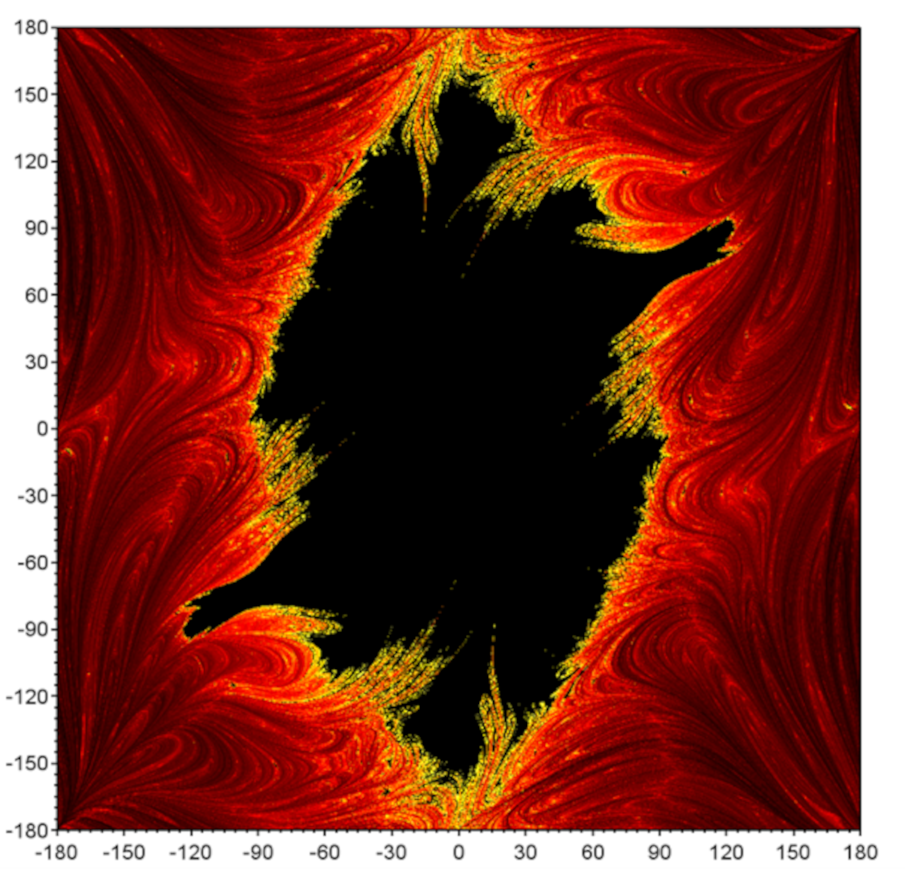
\includegraphics[width=\textwidth]{papers/doppelpendel/images/parameterraum.png}
    \end{minipage}
    \hfill
    \begin{minipage}{0.45\textwidth}
        \centering
        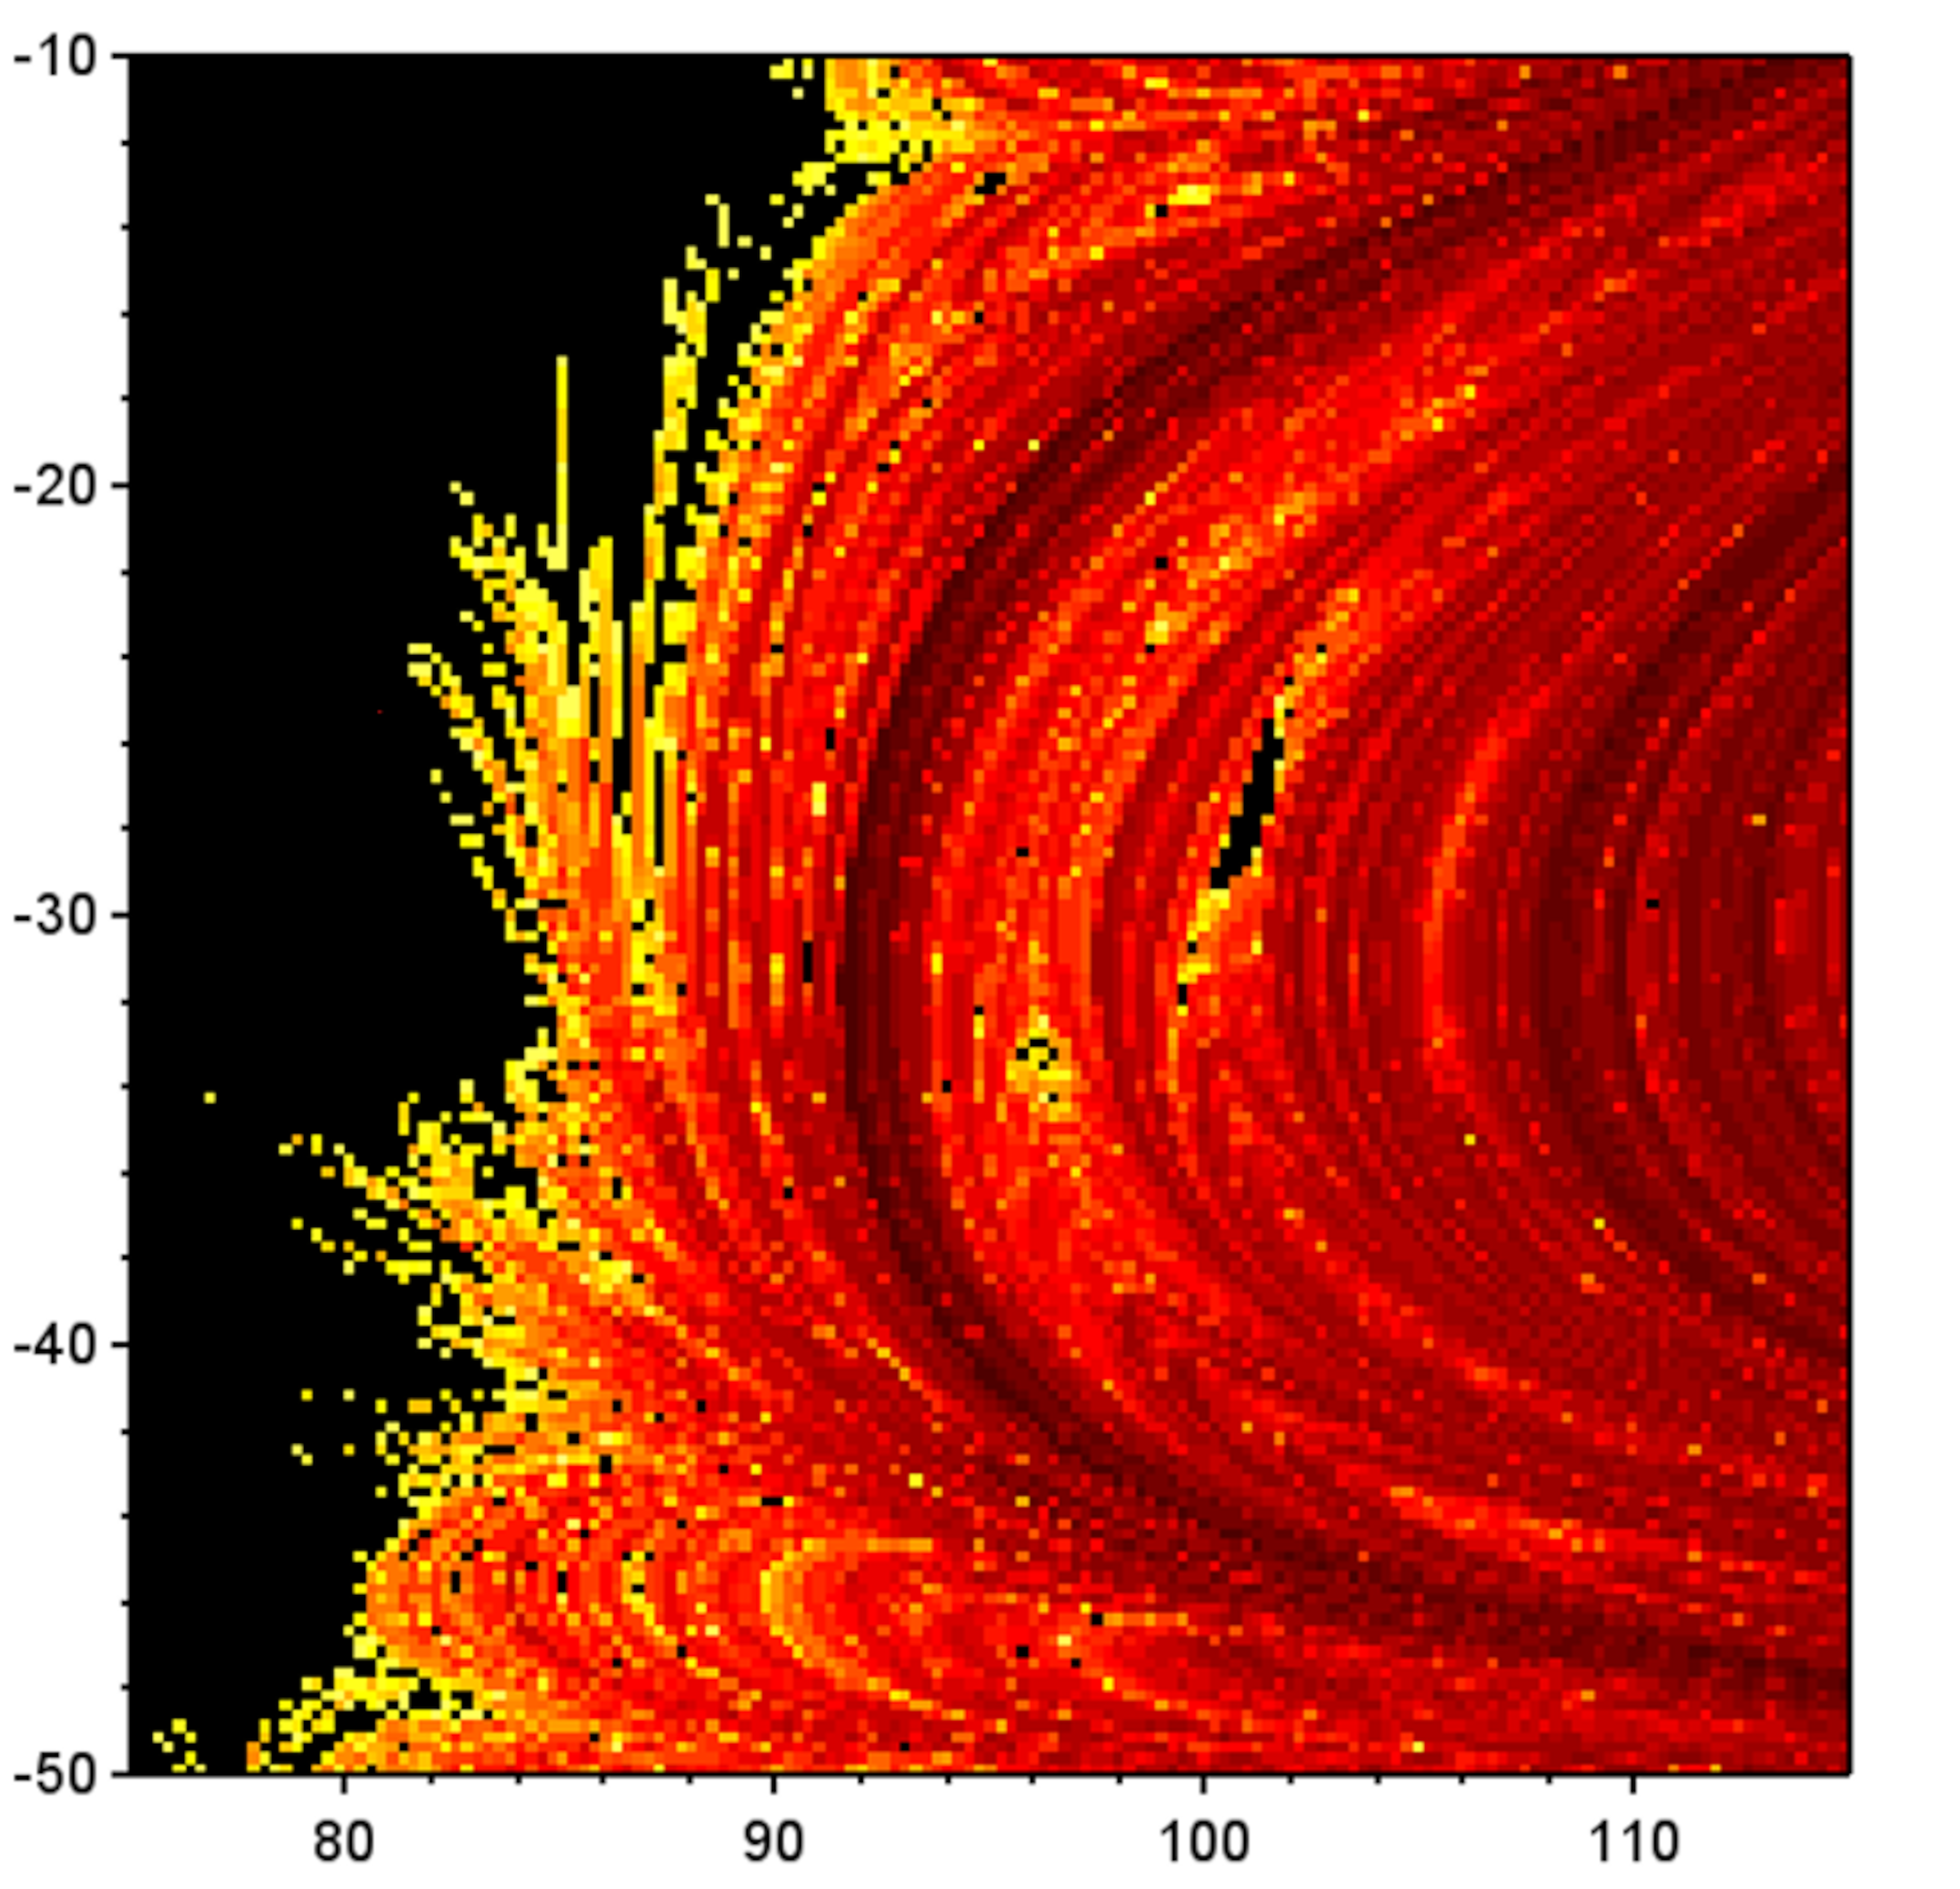
\includegraphics[width=\textwidth]{papers/doppelpendel/images/parameterraum_stabile_inseln.png}
    \end{minipage}
    \caption{Winkelpaare im Parameterraum (links) und stabile Inseln im Parameterraum (rechts)
    \cite{doppelpendel:wettbewerbsarbeit}}
    \label{fig:Parameterraum}
\end{figure}
%
Das wurde durch Davide Farassino bei <<Schweizer Jugend forscht>> 
mithilfe eines Programms untersucht \cite{doppelpendel:wettbewerbsarbeit}.
Das Resultat wurde im sogenannten Parameterraum ausgegeben,
ersichtlich in Abbildung \ref{fig:Parameterraum}.
Auf der horizontalen Achse sind Anfangswinkel von \(\vartheta_1\) und
auf der vertikalen diejenigen von \(\vartheta_2\).
Schwarz bildet die Winkelpaare ab, die nicht ins Chaos übergehen.
Die farbigen Punkte sind daher kritische Winkelpaare.
Es wird unterschieden zwischen dunkelroten Punkten,
das sind Winkelpaare, die schnell chaotisch werden, und
gelben Punkten, die eine kritische Zeit nahe an 30 Sekunden haben.
Äusserst interessant sind die sogenannten stabilen Inseln.
Auch umgeben von kritischen Winkelpaaren, zeigen sich einige
grössere Winkelpaare als nicht kritisch.

Das Resultat der stabilen Winkelpaare aus dem Parameterraum können wir mathematisch noch plausibilisieren.
Wir haben bereits zuvor festgestellt, dass bei kleiner potentieller Energie das System stabil bleibt.
Dies führt zu ebenso kleiner kinetischer Energie, was anders formuliert heisst:
Die Geschwindigkeiten sind vernachlässigbar klein.
Wenn wir in unseren Bewegungsgleichungen
\eqref{eq:bewegungsgleichung1} und \eqref{eq:bewegungsgleichung2}
die Terme höherer Ordnung vernachlässigen, bekommen wir
\begin{align*}
\ddot{\vartheta_1} &= -\frac{g}{l_1} \vartheta_1\\
\ddot{\vartheta_2} &= -\frac{g}{l_2} \vartheta_2
\end{align*}
als lineare Differentialgleichung mit periodischem Verhalten.
Ebenso wurde für kleine Winkel bereits berücksichtigt,
dass \(\sin(\vartheta)\) zu \(\vartheta\) vereinfacht werden kann.

